%==============================================================
%  EE201 -- Circuit Theory I
%  Lecture 3 : Lumped Elements and Their Characteristics
%  M. Mert Ankaralı, METU EEE
%
%  Compile:  ./build.sh      (or: pdflatex EE201_Lecture_3.tex, twice)
%==============================================================
\documentclass[11pt,a4paper]{article}

%-------------------- packages --------------------------------
\usepackage[T1]{fontenc}
\usepackage[utf8]{inputenc}
\usepackage[english]{babel}
\usepackage{lmodern}
\usepackage[margin=2.3cm,top=2.0cm,bottom=1.9cm,headheight=14pt,headsep=9pt]{geometry}
\usepackage{amsmath,amssymb}
\usepackage{array,booktabs,tabularx}
\usepackage{enumitem}
\usepackage[table]{xcolor}
\usepackage{fancyhdr}
\usepackage{titlesec}
\usepackage{graphicx}
\usepackage[most]{tcolorbox}
\usepackage{tikz}
\usepackage[american,siunitx]{circuitikz}
\usetikzlibrary{arrows.meta,positioning,calc,decorations.pathmorphing,decorations.pathreplacing,decorations.markings,patterns,shapes.geometric}
\usepackage[colorlinks=true,allcolors=metured,breaklinks=true]{hyperref}

%-------------------- colour system ---------------------------
% One colour per physical quantity, used identically in the slides.
\definecolor{metured}{RGB}{155,27,48}    % headings, structure
\definecolor{metugray}{RGB}{88,89,91}
\definecolor{ccur}{RGB}{0,102,170}       % CURRENT  -- blue
\definecolor{cvolt}{RGB}{214,120,0}      % VOLTAGE  -- orange
\definecolor{cpow}{RGB}{23,128,74}       % POWER / ENERGY -- green
\definecolor{ccharge}{RGB}{124,60,160}   % CHARGE   -- purple
\definecolor{boxgray}{RGB}{245,245,245}

\newcommand{\Icol}[1]{\textcolor{ccur}{#1}}
\newcommand{\Vcol}[1]{\textcolor{cvolt}{#1}}
\newcommand{\Pcol}[1]{\textcolor{cpow}{#1}}
\newcommand{\Qcol}[1]{\textcolor{ccharge}{#1}}

%-------------------- units (no siunitx dependency) -----------
\newcommand{\uni}[1]{\,\mathrm{#1}}
\newcommand{\A}{\uni{A}}   \newcommand{\V}{\uni{V}}
\newcommand{\W}{\uni{W}}   \newcommand{\J}{\uni{J}}
\newcommand{\Cb}{\uni{C}}  \newcommand{\s}{\uni{s}}

%-------------------- layout ----------------------------------
\pagestyle{fancy}
\fancyhf{}
\lhead{\small\textcolor{metugray}{EE201 -- Circuit Theory I}}
\rhead{\small\textcolor{metugray}{Lecture 3: Lumped Elements}}
\cfoot{\small\thepage}
\renewcommand{\headrulewidth}{0.4pt}

\titleformat{\section}{\large\bfseries\color{metured}}{\thesection.}{0.6em}{}
\titleformat{\subsection}{\normalsize\bfseries\color{metugray}}{\thesubsection.}{0.6em}{}
\titlespacing*{\section}{0pt}{1.4ex plus .3ex}{0.7ex}
\titlespacing*{\subsection}{0pt}{1.1ex plus .2ex}{0.5ex}

\setlist[itemize]{itemsep=2pt,topsep=3pt,parsep=0pt,leftmargin=1.5em}
\setlist[enumerate]{itemsep=2pt,topsep=3pt,parsep=0pt,leftmargin=1.7em}
\setlength{\parindent}{0pt}
\setlength{\parskip}{0.7ex plus .1ex}
\raggedbottom
\widowpenalty=10000
\clubpenalty=10000
\brokenpenalty=10000

%-------------------- boxes -----------------------------------
\newtcolorbox{definitionbox}[1]{enhanced,
  colback=metured!4, colframe=metured, boxrule=0.9pt,
  fonttitle=\bfseries, title={#1}, arc=2pt,
  left=7pt,right=7pt,top=5pt,bottom=5pt, before skip=7pt, after skip=7pt}

\newtcolorbox{ideabox}[1][Key idea]{enhanced,
  colback=ccur!5, colframe=ccur, boxrule=0.9pt,
  fonttitle=\bfseries, title={#1}, arc=2pt,
  left=7pt,right=7pt,top=5pt,bottom=5pt, before skip=7pt, after skip=7pt}

\newtcolorbox{examplebox}[1][Example]{enhanced,
  colback=cpow!4, colframe=cpow, boxrule=0.9pt,
  fonttitle=\bfseries, title={#1}, arc=2pt,
  left=7pt,right=7pt,top=5pt,bottom=5pt, before skip=7pt, after skip=7pt}

\newtcolorbox{cautionbox}[1][Careful]{enhanced,
  colback=cvolt!6, colframe=cvolt, boxrule=0.9pt,
  fonttitle=\bfseries, title={#1}, arc=2pt,
  left=7pt,right=7pt,top=5pt,bottom=5pt, before skip=7pt, after skip=7pt}

%-------------------- circuitikz defaults ---------------------
\ctikzset{bipoles/length=0.9cm, color=black,
          label/align=straight,
          bipoles/vsourceam/height=0.85, bipoles/vsourceam/width=0.85}
\tikzset{
  curarr/.style={-{Stealth[length=2.6mm]}, ccur, very thick},
  volarr/.style={-{Stealth[length=2.6mm]}, cvolt, very thick},
  blk/.style={draw=metugray, fill=boxgray, rounded corners=2pt,
              minimum height=1.25cm, text width=2.9cm, align=center, font=\small},
  flowarr/.style={-{Stealth[length=3mm]}, metured, very thick},
}

%==============================================================

%-------------------- extra macros for this lecture -----------
\newcommand{\ohm}{\,\Omega}
\newcommand{\kohm}{\,\mathrm{k}\Omega}
\newcommand{\Req}{R_{\mathrm{eq}}}
%  v--i axes:  #1 half-width, #2 half-height, #3 caption under the frame
\newcommand{\viaxes}[3]{%
  \draw[vax] (-#1,0) -- (#1,0) node[right=1pt, font=\scriptsize, text=cvolt] {$v$};
  \draw[vax] (0,-#2) -- (0,#2) node[above=1pt, font=\scriptsize, text=ccur] {$i$};
  \node[ttl] at (0,-#2-0.68) {#3};}
\tikzset{
  gnode/.style={circle, fill=metured, inner sep=0pt, minimum size=4.2pt},
  glab/.style={font=\footnotesize, text=metured},
  barr/.style={-{Stealth[length=2.2mm]}, metugray, thick},
  surf/.style={draw=cpow, very thick, dashed, rounded corners=6pt},
  vax/.style={-{Stealth[length=2mm]}, gray!70},
  crv/.style={metured, very thick},
  ttl/.style={font=\scriptsize\bfseries, text=metugray},
  gbr/.style={metugray, thick, postaction={decorate, decoration={markings,
      mark=at position 0.58 with {\arrow{Stealth[length=2.4mm]}}}}},
  pol/.style={font=\small, text=cvolt},
  iar/.style={-{Stealth[length=2.4mm]}, ccur, very thick},
}

%==============================================================
\begin{document}

%-------------------- title block -----------------------------
\begin{center}
\begin{tcolorbox}[enhanced, colback=metured!5, colframe=metured, boxrule=1pt,
                  arc=3pt, left=10pt,right=10pt,top=7pt,bottom=7pt, width=\textwidth]
\begin{center}
  {\small\scshape Middle East Technical University}\\[2pt]
  {\small\scshape Department of Electrical and Electronics Engineering}\\[7pt]
  {\Large\bfseries\color{metured} EE201 -- Circuit Theory I}\\[4pt]
  {\large\bfseries Lecture 3: Lumped Elements and Their Characteristics}\\[6pt]
  {\small M. Mert Ankaralı}
\end{center}
\end{tcolorbox}
\end{center}
\vspace{-0.5em}

\begin{center}
\small
\begin{tabular}{@{}l l@{}}
\toprule
\multicolumn{2}{@{}l}{\textbf{Colour code used in these notes and in the slides}}\\
\midrule
\Qcol{$\blacksquare$}~charge $q$ & \Icol{$\blacksquare$}~current $i$ \quad
\Vcol{$\blacksquare$}~voltage $v$ \quad \Pcol{$\blacksquare$}~power $p$, energy $w$\\
\bottomrule
\end{tabular}
\end{center}

%==============================================================
\section{The other half of the equations}

Lecture~2 gave us the \emph{network} equations: KCL and KVL, which know how the elements
are wired and nothing about what they are. The other half of the $2b$ equations is one
\textbf{terminal equation} per element, and that is where all the physics hides.

\begin{center}
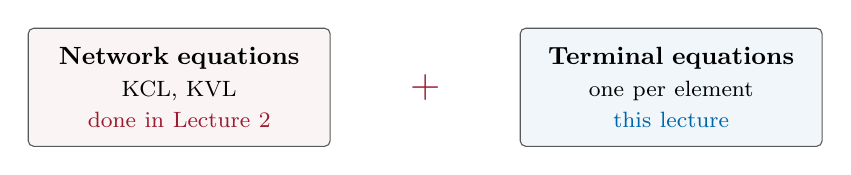
\begin{tikzpicture}[node distance=0.9cm]
  \node[blk, text width=3.6cm, minimum height=1.5cm, fill=metured!5] (n)
       {\textbf{Network equations}\\[2pt]\footnotesize KCL, KVL\\ \footnotesize
        \textcolor{metured}{done in Lecture 2}};
  \node[blk, text width=3.6cm, minimum height=1.5cm, right=2.4cm of n, fill=ccur!6] (t)
       {\textbf{Terminal equations}\\[2pt]\footnotesize one per element\\ \footnotesize
        \textcolor{ccur}{this lecture}};
  \node[font=\Large, text=metured] at ($(n)!0.5!(t)$) {$+$};
\end{tikzpicture}
\end{center}

So far only one element has been given a terminal equation --- the linear resistor,
$\Vcol{v} = R\Icol{i}$. This lecture asks the general question: \emph{what can a
two-terminal element be?}

%==============================================================
\section{An element is a curve in the $v$--$i$ plane}

Take any two-terminal element, attach the reference directions of the passive sign
convention, and watch it. At each instant it has a voltage $\Vcol{v}$ and a current
$\Icol{i}$ --- one point in a plane.

\begin{center}
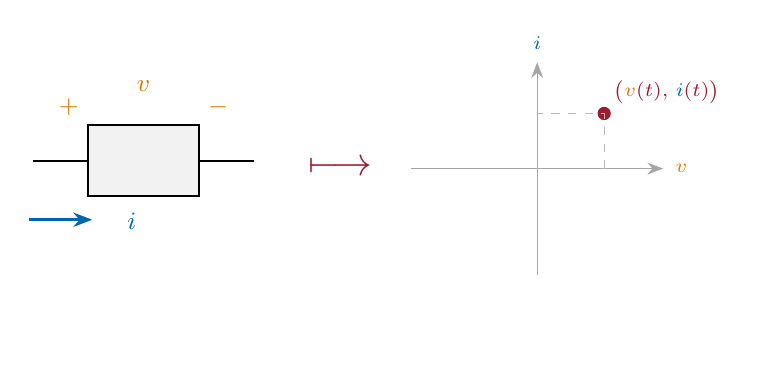
\begin{tikzpicture}[scale=1.0]
%---- element with PSC references
\begin{scope}[yshift=0.1cm]
  \draw[thick] (0,0) -- (0.7,0); \draw[thick] (2.1,0) -- (2.8,0);
  \draw[thick, fill=gray!10] (0.7,-0.45) rectangle (2.1,0.45);
  \node[pol] at (0.45,0.68) {$+$}; \node[pol] at (2.35,0.68) {$-$};
  \node[pol] at (1.4,0.95) {$v$};
  \draw[iar] (-0.05,-0.75) -- (0.75,-0.75);
  \node[ccur, font=\small] at (1.25,-0.77) {$i$};
\end{scope}
\node[font=\Large, text=metured] at (3.9,0) {$\longmapsto$};
%---- the plane
\begin{scope}[xshift=6.4cm]
  \viaxes{1.6}{1.35}{}
  \fill[metured] (0.85,0.7) circle (2.4pt);
  \node[font=\scriptsize, text=metured, above right=0pt] at (0.85,0.7)
       {$\big(\Vcol{v}(t),\,\Icol{i}(t)\big)$};
  \draw[gray!55, dashed] (0.85,0) -- (0.85,0.7) -- (0,0.7);
\end{scope}
\end{tikzpicture}
\end{center}

As time passes the point moves. The element is defined by \emph{which points it is allowed
to visit}.

\begin{definitionbox}{Characteristic}
The \textbf{characteristic} of a two-terminal element is the collection of \emph{all} the
pairs $(\Vcol{v},\Icol{i})$ that the element allows. Drawn in the plane, it is a
\textbf{curve}: the operating point may sit anywhere on that curve and nowhere else.
\\[3pt]
Everything the element does is in that picture; nothing else about it matters to circuit
theory. If the curve itself changes with time we write it as the curve \emph{at time $t$}.
\end{definitionbox}

\begin{center}
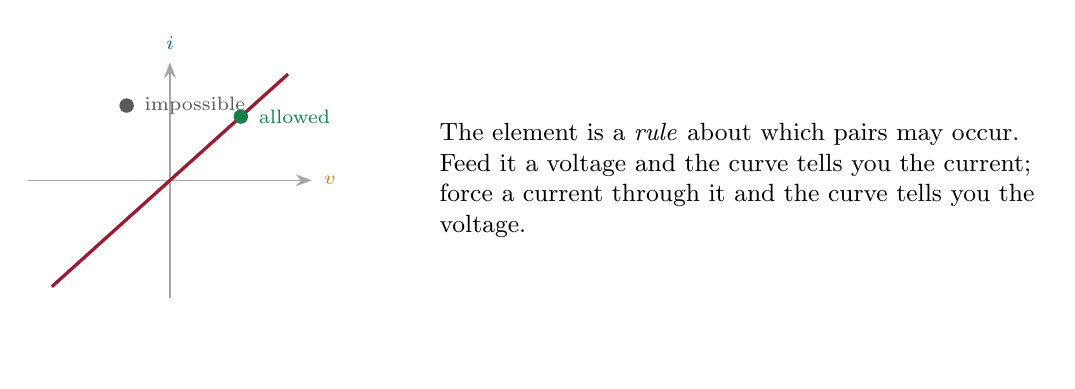
\begin{tikzpicture}[scale=1.0]
  \viaxes{1.8}{1.5}{}
  \draw[crv] (-1.5,-1.35) -- (1.5,1.35);
  \fill[cpow] (0.9,0.81) circle (2.6pt);
  \node[font=\scriptsize, text=cpow, right=3pt] at (0.9,0.81) {allowed};
  \fill[metugray] (-0.55,0.95) circle (2.6pt);
  \node[font=\scriptsize, text=metugray, right=3pt] at (-0.55,0.95) {impossible};
  \node[font=\small, anchor=west, text width=7.6cm] at (3.3,0)
    {The element is a \emph{rule} about which pairs may occur. Feed it a voltage and the
     curve tells you the current; force a current through it and the curve tells you the
     voltage.};
\end{tikzpicture}
\end{center}

\begin{ideabox}[Every element is a curve]
A linear resistor is a straight line through the origin. A battery is a vertical line. A
diode is a bent curve.\\[3pt]
For every new element, we ask the same thing: \emph{which curve?} Section~\ref{sec:words}
is about the shape of that curve and nothing else.
\end{ideabox}

%==============================================================
\section{The independent voltage source}

\begin{definitionbox}{Independent voltage source}
An element whose terminal voltage is a prescribed function of time, \emph{whatever current
flows through it}:
\[
  \Vcol{v(t)} = v_s(t) \qquad\text{for every } \Icol{i} .
\]
Its characteristic at time $t$ is the \textbf{vertical line} $\Vcol{v} = v_s(t)$.
\end{definitionbox}

\begin{center}
\begin{tikzpicture}[scale=1.0]
\begin{scope}[yshift=-0.1cm]
  \draw (0,0) to[american voltage source, invert] (0,2.0);
  \node[pol] at (0.68,1.42) {$+$}; \node[pol] at (0.68,0.52) {$-$};
  \node[pol] at (1.02,0.97) {$v$};
  \draw[iar] (-0.62,0.62) -- (-0.62,1.32); \node[ccur, font=\small] at (-0.95,0.97) {$i$};
  \node[font=\footnotesize, text=metugray] at (0.0,-0.75) {$\Vcol{v} = v_s(t)$};
\end{scope}
\node[font=\Large, text=metured] at (2.1,0.9) {$\longmapsto$};
\begin{scope}[xshift=4.6cm, yshift=0.9cm]
  \viaxes{1.5}{1.3}{}
  \draw[crv] (0.75,-1.2) -- (0.75,1.2);
  \node[font=\scriptsize, text=cvolt] at (1.12,-0.85) {$v_s$};
  \draw[-{Stealth[length=1.8mm]}, gray!70] (0.75,0.55) -- (1.25,0.55);
  \node[font=\tiny, text=metugray, right] at (1.28,0.55) {$v_s$ may move with $t$};
\end{scope}
\begin{scope}[xshift=9.9cm, yshift=0.9cm]
  \viaxes{1.5}{1.3}{}
  \draw[crv] (0,-1.2) -- (0,1.2);
  \node[font=\scriptsize\bfseries, text=metugray] at (0,-1.75) {$v_s = 0$: a short circuit};
\end{scope}
\end{tikzpicture}
\end{center}
\vspace{2pt}

\subsection{Two symbols, one element}

\begin{center}
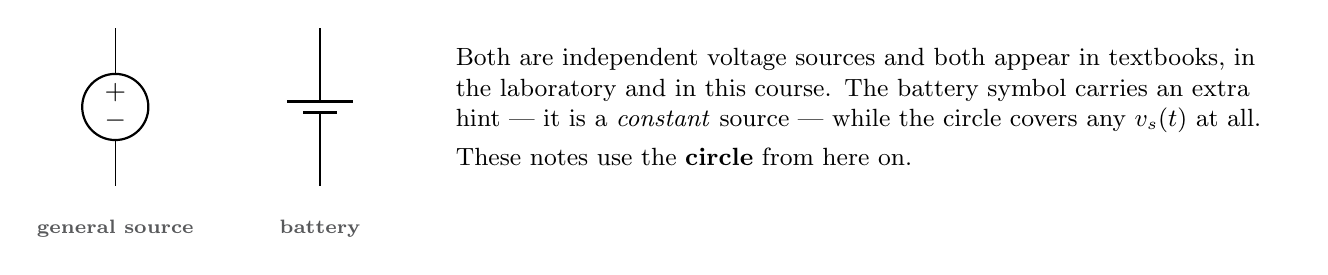
\begin{tikzpicture}[scale=1.0]
  \begin{scope}
    \draw (0,0) to[american voltage source, invert] (0,2.0);
    \node[ttl] at (0,-0.55) {general source};
  \end{scope}
  \begin{scope}[xshift=2.6cm]
    \draw (0,0) to[battery1, invert] (0,2.0);
    \node[ttl] at (0,-0.55) {battery};
  \end{scope}
  \node[font=\small, anchor=west, text width=10.6cm] at (4.2,1.0)
    {Both are independent voltage sources and both appear in textbooks, in the laboratory
     and in this course. The battery symbol carries an extra hint --- it is a
     \emph{constant} source --- while the circle covers any $v_s(t)$ at all. \\[3pt]
     These notes use the \textbf{circle} from here on.};
\end{tikzpicture}
\end{center}

\begin{cautionbox}[A voltage source does not decide the current]
The line is vertical precisely because $\Icol{i}$ is \emph{unconstrained} by the element:
the source will supply whatever current the rest of the circuit demands at that voltage.
Which current actually flows is settled by KCL, KVL and the other elements --- never by
the source alone.
\end{cautionbox}

\subsection{Waveforms}

$v_s(t)$ is any function you like; these four cover most of this course.

\begin{center}
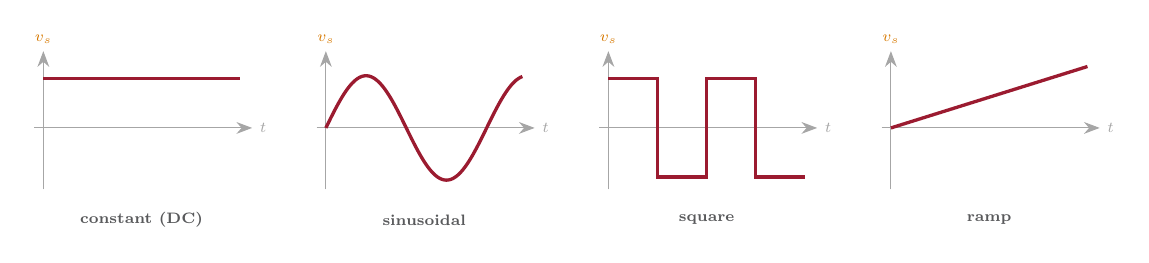
\begin{tikzpicture}[scale=0.78, transform shape]
 \foreach \dx/\ttl in {0/{constant (DC)}, 4.6/{sinusoidal}, 9.2/{square}, 13.8/{ramp}}{
   \begin{scope}[xshift=\dx cm]
     \draw[vax] (-0.15,0) -- (3.4,0) node[right, font=\scriptsize] {$t$};
     \draw[vax] (0,-1.0) -- (0,1.25) node[above, font=\scriptsize, text=cvolt] {$v_s$};
     \node[ttl] at (1.6,-1.5) {\ttl};
   \end{scope}}
 \draw[crv] (0,0.8) -- (3.2,0.8);
 \begin{scope}[xshift=4.6cm]
   \draw[crv, domain=0:3.2, samples=120, smooth] plot (\x, {0.85*sin(deg(2.4*\x))});
 \end{scope}
 \begin{scope}[xshift=9.2cm]
   \draw[crv] (0,0.8)--(0.8,0.8)--(0.8,-0.8)--(1.6,-0.8)--(1.6,0.8)--(2.4,0.8)
              --(2.4,-0.8)--(3.2,-0.8);
 \end{scope}
 \begin{scope}[xshift=13.8cm]
   \draw[crv] (0,0) -- (3.2,1.0);
 \end{scope}
\end{tikzpicture}
\end{center}
\vspace{4pt}

\begin{examplebox}[Example 3.1 --- the source does not act alone]
A $12\V$ source is connected first to a $4\ohm$ resistor, then to a $2\ohm$ one.
\[
  \Icol{i} = \frac{12}{4} = 3\A , \qquad\qquad \Icol{i} = \frac{12}{2} = 6\A .
\]
The source's characteristic never changed --- it is the same vertical line at
$\Vcol{v} = 12\V$. What changed is the \emph{other} element's line, and with it the point
where the two characteristics meet. Section~\ref{sec:loadline} makes that picture explicit.
\end{examplebox}

%==============================================================
\section{The independent current source}

Everything above, with $\Vcol{v}$ and $\Icol{i}$ exchanged.

\begin{definitionbox}{Independent current source}
An element whose terminal current is a prescribed function of time, \emph{whatever voltage
appears across it}:
\[
  \Icol{i(t)} = i_s(t) \qquad\text{for every } \Vcol{v} .
\]
Its characteristic at time $t$ is the \textbf{horizontal line} $\Icol{i} = i_s(t)$.
\end{definitionbox}

\begin{center}
\begin{tikzpicture}[scale=1.0]
\begin{scope}[yshift=-0.1cm]
  \draw (0,0) to[american current source] (0,2.0);
  \node[pol] at (0.42,1.42) {$+$}; \node[pol] at (0.42,0.52) {$-$};
  \node[pol] at (0.76,0.97) {$v$};
  \draw[iar] (-0.55,0.62) -- (-0.55,1.32); \node[ccur, font=\small] at (-0.88,0.97) {$i$};
  \node[font=\footnotesize, text=metugray] at (0.0,-0.75) {$\Icol{i} = i_s(t)$};
\end{scope}
\node[font=\Large, text=metured] at (2.1,0.9) {$\longmapsto$};
\begin{scope}[xshift=4.6cm, yshift=0.9cm]
  \viaxes{1.5}{1.3}{}
  \draw[crv] (-1.35,0.65) -- (1.35,0.65);
  \node[font=\scriptsize, text=ccur] at (-1.0,0.95) {$i_s$};
\end{scope}
\begin{scope}[xshift=9.9cm, yshift=0.9cm]
  \viaxes{1.5}{1.3}{}
  \draw[crv] (-1.35,0) -- (1.35,0);
  \node[font=\scriptsize\bfseries, text=metugray] at (0,-1.75) {$i_s = 0$: an open circuit};
\end{scope}
\end{tikzpicture}
\end{center}
\vspace{2pt}

\begin{cautionbox}[The dual warning]
A current source does not decide its voltage. Connect $2\A$ to $4\ohm$ and it produces
$8\V$; connect it to $100\ohm$ and it produces $200\V$; leave it open-circuited and the
ideal model demands infinite voltage --- which is the model telling you that a real current
source has a limit, and beyond it something gives way.
\end{cautionbox}

%==============================================================
\section{Sources are active}

With the passive sign convention, $\Pcol{p} = \Vcol{v}\Icol{i}$ is the power \emph{absorbed}.
So the sign of $\Pcol{p}$ is decided by which quadrant of the $v$--$i$ plane the operating
point sits in.

\begin{center}
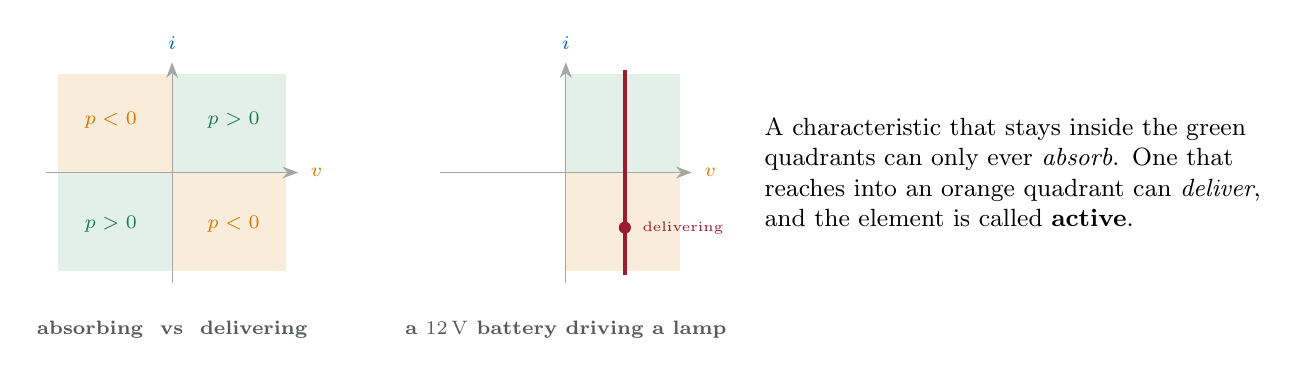
\begin{tikzpicture}[scale=1.0]
\begin{scope}
  \fill[cpow!12] (0,0) rectangle (1.45,1.25);
  \fill[cpow!12] (0,0) rectangle (-1.45,-1.25);
  \fill[cvolt!14] (0,0) rectangle (-1.45,1.25);
  \fill[cvolt!14] (0,0) rectangle (1.45,-1.25);
  \viaxes{1.6}{1.4}{}
  \node[font=\scriptsize, text=cpow] at (0.78,0.66) {$p > 0$};
  \node[font=\scriptsize, text=cpow] at (-0.78,-0.66) {$p > 0$};
  \node[font=\scriptsize, text=cvolt] at (-0.78,0.66) {$p < 0$};
  \node[font=\scriptsize, text=cvolt] at (0.78,-0.66) {$p < 0$};
  \node[ttl] at (0,-2.0) {absorbing \ vs \ delivering};
\end{scope}
\begin{scope}[xshift=5.0cm]
  \fill[cvolt!14] (0,0) rectangle (1.45,-1.25);
  \fill[cpow!12] (0,0) rectangle (1.45,1.25);
  \viaxes{1.6}{1.4}{}
  \draw[crv] (0.75,-1.3) -- (0.75,1.3);
  \fill[metured] (0.75,-0.7) circle (2.2pt);
  \node[font=\tiny, text=metured, right=2pt] at (0.78,-0.7) {delivering};
  \node[ttl] at (0,-2.0) {a $12\V$ battery driving a lamp};
\end{scope}
\node[font=\small, anchor=west, text width=6.4cm] at (7.4,0)
  {A characteristic that stays inside the green quadrants can only ever \emph{absorb}.
   One that reaches into an orange quadrant can \emph{deliver}, and the element is called
   \textbf{active}.};
\end{tikzpicture}
\end{center}
\vspace{2pt}

\begin{definitionbox}{Passive and active}
An element is \textbf{passive} if its characteristic lies entirely in the first and third
quadrants at every instant, so that $\Pcol{p} = \Vcol{v}\Icol{i} \ge 0$ always. Otherwise
it is \textbf{active}.
\end{definitionbox}

A voltage source with $v_s \neq 0$ is a vertical line that crosses both the first and the
fourth quadrant, so it is active --- as it must be, since driving a circuit means giving
out energy. The same argument makes any current source with $i_s \neq 0$ active. Short
circuits, open circuits and positive resistances are passive.

%==============================================================
\section{The resistor --- a much larger family than you expect}

\begin{definitionbox}{Resistor}
A two-terminal element is a \textbf{resistor} if, at every instant, its characteristic is a
curve in the $\Vcol{v}$--$\Icol{i}$ plane.
\end{definitionbox}

Read that carefully: it says nothing about straight lines, nothing about Ohm's law, and
nothing about $R$. What it does say is that the relation between $\Vcol{v}$ and $\Icol{i}$
is \emph{purely algebraic} --- no derivatives, no integrals, no memory of what happened a
moment ago. The present current depends only on the present voltage and vice versa.

\begin{ideabox}[Consequences worth pausing over]
\begin{itemize}
  \item A $pn$ junction diode is a resistor. So is a tunnel diode, a light bulb, a
        thermistor.
  \item A short circuit and an open circuit are resistors.
  \item An \emph{independent source} is a resistor too --- its characteristic is a
        straight line, just not through the origin.
  \item Capacitors and inductors are \textbf{not} resistors: $\Icol{i} = C\,d\Vcol{v}/dt$
        is not a curve in the $v$--$i$ plane, because the same $\Vcol{v}$ allows any
        $\Icol{i}$ depending on how $\Vcol{v}$ is changing.
\end{itemize}
The linear resistor of Lecture~1 is one member of this family --- the straight line through
the origin --- and it is only the simplest.
\end{ideabox}

Yes, that really does make a battery a resistor. The word here describes the \emph{shape of
the relation} --- algebraic, memoryless --- and says nothing about dissipating energy;
active elements qualify just as well as passive ones. If it helps, read ``resistor'' as
``memoryless element'' every time.

\subsection{A gallery}

\begin{center}
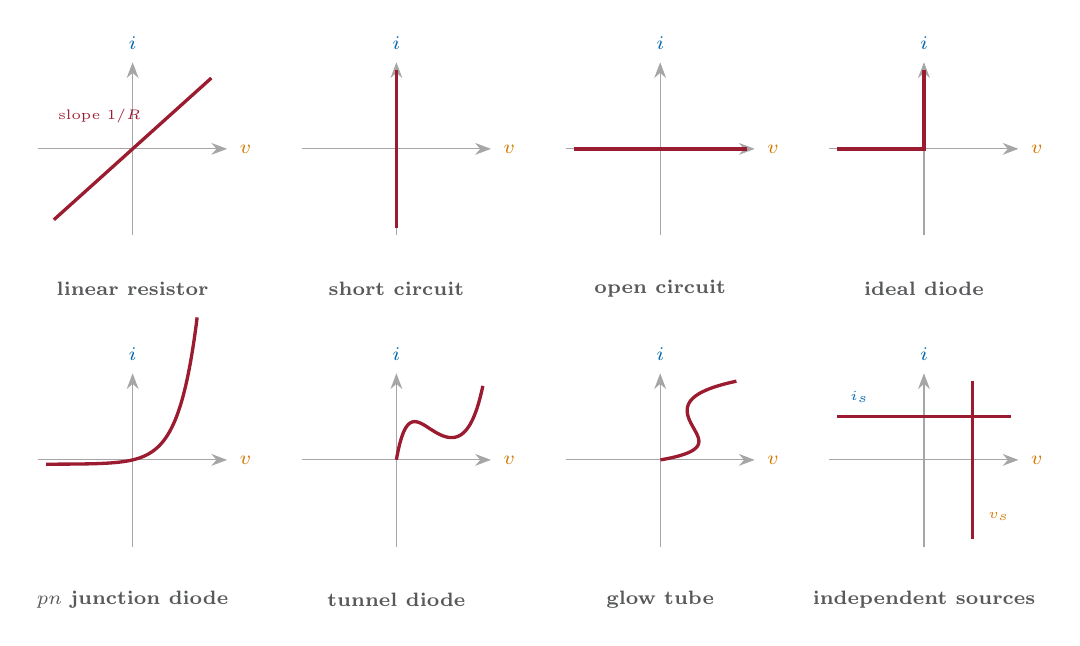
\begin{tikzpicture}[x=1cm,y=1cm]
\def\W{1.2} \def\H{1.1} \def\S{3.35}
\begin{scope}
  \viaxes{\W}{\H}{linear resistor}
  \draw[crv] (-1.0,-0.9) -- (1.0,0.9);
  \node[font=\tiny, text=metured] at (-0.42,0.42) {slope $1/R$};
\end{scope}
\begin{scope}[xshift=\S cm]
  \viaxes{\W}{\H}{short circuit}
  \draw[crv] (0,-1.0) -- (0,1.0);
\end{scope}
\begin{scope}[xshift=2*\S cm]
  \viaxes{\W}{\H}{open circuit}
  \draw[crv] (-1.1,0) -- (1.1,0);
\end{scope}
\begin{scope}[xshift=3*\S cm]
  \viaxes{\W}{\H}{ideal diode}
  \draw[crv] (-1.1,0) -- (0,0) -- (0,1.0);
\end{scope}
\begin{scope}[yshift=-3.95cm]
  \viaxes{\W}{\H}{$pn$ junction diode}
  \draw[crv, domain=-1.1:0.82, samples=140, smooth] plot (\x, {0.055*(exp(4.3*\x)-1)});
\end{scope}
\begin{scope}[xshift=\S cm, yshift=-3.95cm]
  \viaxes{\W}{\H}{tunnel diode}
  \draw[crv, domain=0:1.1, samples=180, smooth]
       plot (\x, {5.72*\x*exp(-4.4*\x) + 0.9*exp(5.5*(\x-1.1))});
\end{scope}
\begin{scope}[xshift=2*\S cm, yshift=-3.95cm]
  \viaxes{\W}{\H}{glow tube}
  \draw[crv, domain=0:1.0, samples=180, smooth]
       plot ({5.72*\x*exp(-4.4*\x) + 0.9*exp(5.5*(\x-1.0))}, \x);
\end{scope}
\begin{scope}[xshift=3*\S cm, yshift=-3.95cm]
  \viaxes{\W}{\H}{independent sources}
  \draw[crv] (0.62,-1.0) -- (0.62,1.0);
  \draw[crv] (-1.1,0.55) -- (1.1,0.55);
  \node[font=\tiny, text=cvolt] at (0.95,-0.72) {$v_s$};
  \node[font=\tiny, text=ccur] at (-0.82,0.8) {$i_s$};
\end{scope}
\end{tikzpicture}
\end{center}

%==============================================================
\section{Five words for describing a resistor}
\label{sec:words}

Every one of them is a statement about the \emph{shape} of the characteristic.

\subsection{Linear}

\begin{definitionbox}{Linear}
The characteristic is a \textbf{straight line through the origin}. Equivalently,
superposition holds: scaling $\Vcol{v}$ by $\alpha$ scales $\Icol{i}$ by the same
$\alpha$.
\end{definitionbox}

\begin{center}
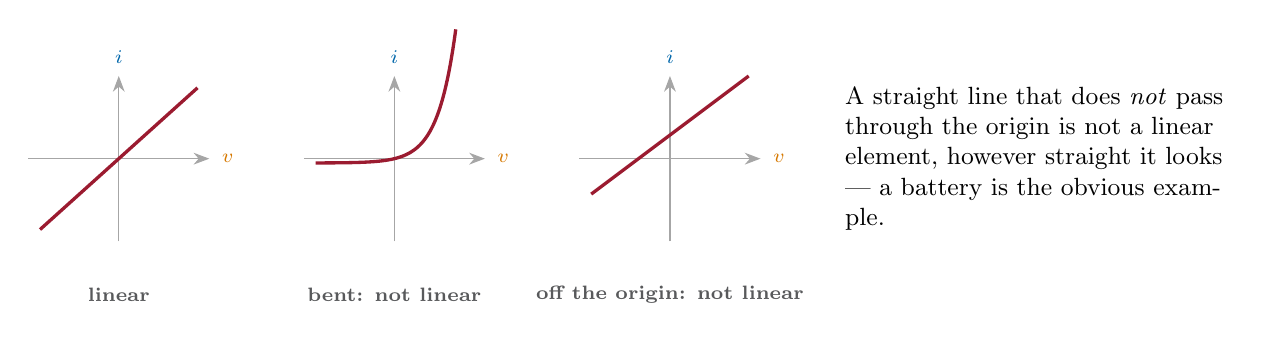
\begin{tikzpicture}[x=1cm,y=1cm]
\def\W{1.15} \def\H{1.05}
\begin{scope}
  \viaxes{\W}{\H}{linear}
  \draw[crv] (-1.0,-0.9) -- (1.0,0.9);
\end{scope}
\begin{scope}[xshift=3.5cm]
  \viaxes{\W}{\H}{bent: not linear}
  \draw[crv, domain=-1.0:0.78, samples=140, smooth] plot (\x, {0.055*(exp(4.4*\x)-1)});
\end{scope}
\begin{scope}[xshift=7.0cm]
  \viaxes{\W}{\H}{off the origin: not linear}
  \draw[crv] (-1.0,-0.45) -- (1.0,1.05);
\end{scope}
\node[font=\small, anchor=west, text width=5.0cm] at (9.1,0)
  {A straight line that does \emph{not} pass through the origin is not a linear element,
   however straight it looks --- a battery is the obvious example.};
\end{tikzpicture}
\end{center}

\subsection{Bilateral}

\begin{definitionbox}{Bilateral}
The characteristic is \textbf{symmetric about the origin}: whenever the pair
$(\Vcol{v},\Icol{i})$ is on the curve, so is $(-\Vcol{v},\,-\Icol{i})$.
Physically: swapping the two terminals round makes no difference.
\end{definitionbox}

\begin{center}
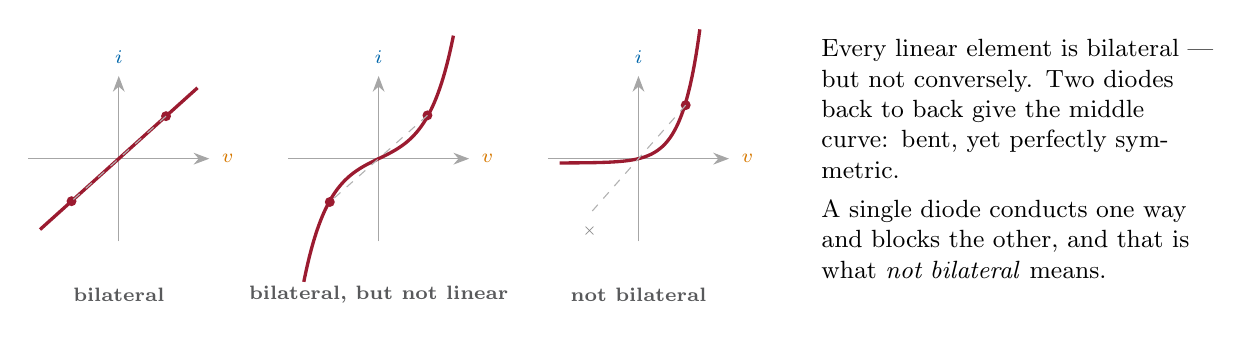
\begin{tikzpicture}[x=1cm,y=1cm]
\def\W{1.15} \def\H{1.05}
\begin{scope}
  \viaxes{\W}{\H}{bilateral}
  \draw[crv] (-1.0,-0.9) -- (1.0,0.9);
  \fill[metured] (0.6,0.54) circle (1.8pt); \fill[metured] (-0.6,-0.54) circle (1.8pt);
  \draw[gray!60, dashed] (0.6,0.54) -- (-0.6,-0.54);
\end{scope}
\begin{scope}[xshift=3.3cm]
  \viaxes{\W}{\H}{bilateral, but not linear}
  \draw[crv, domain=-0.95:0.95, samples=160, smooth]
       plot (\x, {0.075*(exp(3.2*\x)-exp(-3.2*\x))});
  \fill[metured] (0.62,0.55) circle (1.8pt); \fill[metured] (-0.62,-0.55) circle (1.8pt);
  \draw[gray!60, dashed] (0.62,0.55) -- (-0.62,-0.55);
\end{scope}
\begin{scope}[xshift=6.6cm]
  \viaxes{\W}{\H}{not bilateral}
  \draw[crv, domain=-1.0:0.78, samples=140, smooth] plot (\x, {0.055*(exp(4.4*\x)-1)});
  \fill[metured] (0.6,0.68) circle (1.8pt);
  \draw[gray!60, dashed] (0.6,0.68) -- (-0.6,-0.68);
  \node[gray, font=\tiny] at (-0.62,-0.92) {$\times$};
\end{scope}
\node[font=\small, anchor=west, text width=5.0cm] at (8.8,0)
  {Every linear element is bilateral --- but not conversely. Two diodes back to back give
   the middle curve: bent, yet perfectly symmetric.\\[3pt]
   A single diode conducts one way and blocks the other, and that is what \emph{not
   bilateral} means.};
\end{tikzpicture}
\end{center}

\subsection{Active or passive}

Defined in Section~5: passive when the characteristic never leaves the first and third
quadrants, so the element can only absorb. Independent sources are active; a positive
linear resistance, a short and an open are passive. A \emph{negative} resistance --- a
straight line through the origin with negative slope --- is a line in the second and
fourth quadrants, and so is active.

\subsection{Voltage-controlled and current-controlled}

\begin{definitionbox}{Controlled by which variable?}
A resistor is \textbf{voltage-controlled} if its characteristic can be written
$\Icol{i} = f(\Vcol{v})$ --- one current for each voltage --- and
\textbf{current-controlled} if it can be written $\Vcol{v} = g(\Icol{i})$. It may be
both, either, or neither.
\end{definitionbox}

\begin{center}
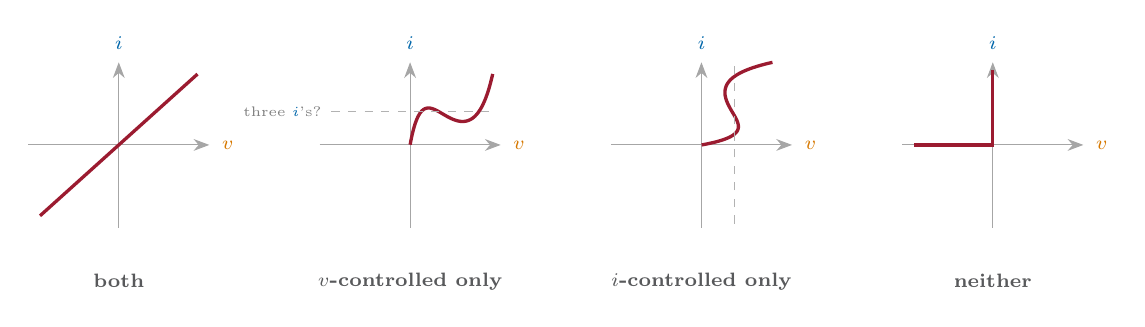
\begin{tikzpicture}[x=1cm,y=1cm]
\def\W{1.15} \def\H{1.05} \def\S{3.7}
\begin{scope}
  \viaxes{\W}{\H}{both}
  \draw[crv] (-1.0,-0.9) -- (1.0,0.9);
\end{scope}
\begin{scope}[xshift=\S cm]
  \viaxes{\W}{\H}{$v$-controlled only}
  \draw[crv, domain=0:1.05, samples=180, smooth]
       plot (\x, {5.5*\x*exp(-4.4*\x) + 0.85*exp(5.5*(\x-1.05))});
  \draw[gray!60, dashed] (-1.0,0.42) -- (1.05,0.42);
  \node[gray, font=\tiny, left] at (-1.0,0.42) {three $\Icol{i}$'s?};
\end{scope}
\begin{scope}[xshift=2*\S cm]
  \viaxes{\W}{\H}{$i$-controlled only}
  \draw[crv, domain=0:1.05, samples=180, smooth]
       plot ({5.5*\x*exp(-4.4*\x) + 0.85*exp(5.5*(\x-1.05))}, \x);
  \draw[gray!60, dashed] (0.42,-1.0) -- (0.42,1.05);
\end{scope}
\begin{scope}[xshift=3*\S cm]
  \viaxes{\W}{\H}{neither}
  \draw[crv] (-1.0,0) -- (0,0) -- (0,0.95);
\end{scope}
\end{tikzpicture}
\end{center}
\vspace{2pt}

For the tunnel diode the dashed horizontal line meets the curve three times: one voltage
per current is impossible, so it is \emph{not} current-controlled, while
$\Icol{i} = f(\Vcol{v})$ is perfectly well defined. The glow tube is the mirror image. The
ideal diode fails both tests: at $\Vcol{v} = 0$ any positive current is allowed, and at
$\Icol{i} = 0$ any negative voltage is.

\subsection{Time-invariant}

\begin{definitionbox}{Time-invariant}
The characteristic is \textbf{the same curve at every instant}. If it moves, stretches or
tilts as $t$ runs, the element is time-varying.
\end{definitionbox}

\begin{center}
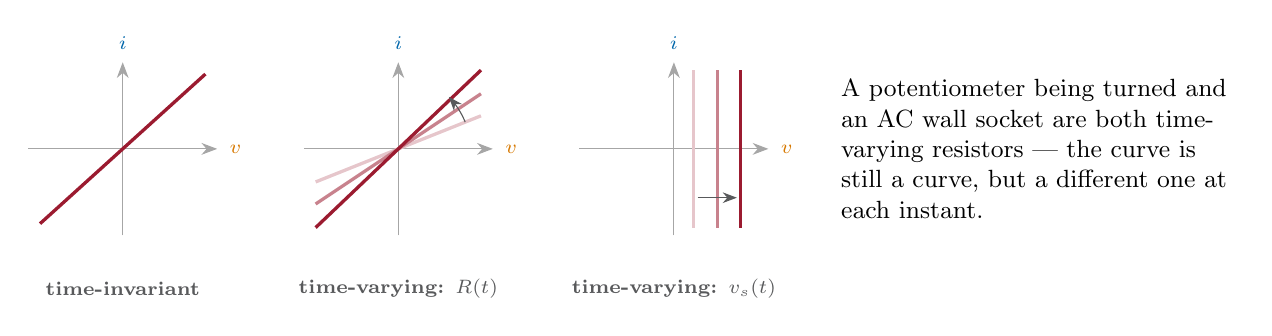
\begin{tikzpicture}[x=1cm,y=1cm]
\def\W{1.2} \def\H{1.1}
\begin{scope}
  \viaxes{\W}{\H}{time-invariant}
  \draw[crv] (-1.05,-0.95) -- (1.05,0.95);
\end{scope}
\begin{scope}[xshift=3.5cm]
  \viaxes{\W}{\H}{time-varying: $R(t)$}
  \draw[metured!25, very thick] (-1.05,-0.42) -- (1.05,0.42);
  \draw[metured!55, very thick] (-1.05,-0.7) -- (1.05,0.7);
  \draw[crv] (-1.05,-1.0) -- (1.05,1.0);
  \draw[-{Stealth[length=1.8mm]}, metugray] (0.85,0.34) arc (22:44:1.0);
\end{scope}
\begin{scope}[xshift=7.0cm]
  \viaxes{\W}{\H}{time-varying: $v_s(t)$}
  \draw[metured!25, very thick] (0.25,-1.0) -- (0.25,1.0);
  \draw[metured!55, very thick] (0.55,-1.0) -- (0.55,1.0);
  \draw[crv] (0.85,-1.0) -- (0.85,1.0);
  \draw[-{Stealth[length=1.8mm]}, metugray] (0.3,-0.62) -- (0.8,-0.62);
\end{scope}
\node[font=\small, anchor=west, text width=5.0cm] at (9.0,0)
  {A potentiometer being turned and an AC wall socket are both time-varying resistors ---
   the curve is still a curve, but a different one at each instant.};
\end{tikzpicture}
\end{center}

%==============================================================
\section{The gallery, characterized}

\begin{center}
\small
\renewcommand{\arraystretch}{1.25}
\begin{tabular}{@{}l c c c c c c@{}}
\toprule
\textbf{Element} & \textbf{linear} & \textbf{bilateral} & \textbf{passive} &
\textbf{$v$-contr.} & \textbf{$i$-contr.} & \textbf{time-inv.}\\
\midrule
linear resistor, $R>0$        & yes & yes & yes & yes & yes & yes\\
linear resistor, $R<0$        & yes & yes & \textcolor{metured}{no}  & yes & yes & yes\\
short circuit                 & yes & yes & yes & \textcolor{metured}{no}  & yes & yes\\
open circuit                  & yes & yes & yes & yes & \textcolor{metured}{no}  & yes\\
ideal diode                   & \textcolor{metured}{no}  & \textcolor{metured}{no}  & yes & \textcolor{metured}{no}  & \textcolor{metured}{no}  & yes\\
$pn$ junction diode           & \textcolor{metured}{no}  & \textcolor{metured}{no}  & yes & yes & yes & yes\\
tunnel diode                  & \textcolor{metured}{no}  & \textcolor{metured}{no}  & yes & yes & \textcolor{metured}{no}  & yes\\
glow tube                     & \textcolor{metured}{no}  & \textcolor{metured}{no}  & yes & \textcolor{metured}{no}  & yes & yes\\
DC voltage source, $v_s\neq0$ & \textcolor{metured}{no}  & \textcolor{metured}{no}  & \textcolor{metured}{no}  & \textcolor{metured}{no}  & yes & yes\\
DC current source, $i_s\neq0$ & \textcolor{metured}{no}  & \textcolor{metured}{no}  & \textcolor{metured}{no}  & yes & \textcolor{metured}{no}  & yes\\
AC voltage source             & \textcolor{metured}{no}  & \textcolor{metured}{no}  & \textcolor{metured}{no}  & \textcolor{metured}{no}  & yes & \textcolor{metured}{no}\\
\bottomrule
\end{tabular}
\end{center}

Three rows are worth checking by eye rather than trusting.

\begin{examplebox}[Example 3.2 --- reading three rows off the pictures]
\textbf{The short circuit} is the line $\Vcol{v} = 0$. Ask for $\Icol{i} = f(\Vcol{v})$:
at $\Vcol{v} = 0$ every current is allowed, so no function exists --- not
voltage-controlled. Ask for $\Vcol{v} = g(\Icol{i})$: $g(\Icol{i}) = 0$ for every
$\Icol{i}$ --- current-controlled. The open circuit is the mirror image.
\vspace{3pt}

\textbf{The $pn$ diode}, $\Icol{i} = I_s(e^{\Vcol{v}/V_T} - 1)$, is a single-valued
increasing function both ways round, so it is voltage- \emph{and} current-controlled. Its
curve stays in quadrants~1 and~3, so it is passive; it is bent, so nonlinear; and it is
not symmetric about the origin, so not bilateral.
\vspace{3pt}

\textbf{The DC voltage source} is a vertical line at $\Vcol{v} = v_s$. It is not linear
(misses the origin), not bilateral, not passive (it reaches quadrant~4), not
voltage-controlled (at $\Vcol{v} = v_s$ any current is allowed) --- but it is
current-controlled, since $\Vcol{v} = v_s$ for every $\Icol{i}$.
\end{examplebox}

%==============================================================
\section{Why the picture was worth drawing}
\label{sec:loadline}

Two elements joined face to face must agree: KCL forces one current through both, KVL
forces one voltage across both, so the pair $(\Vcol{v},\Icol{i})$ has to lie on
\emph{both} characteristics at once. The operating point is where the two curves cross.

\begin{center}
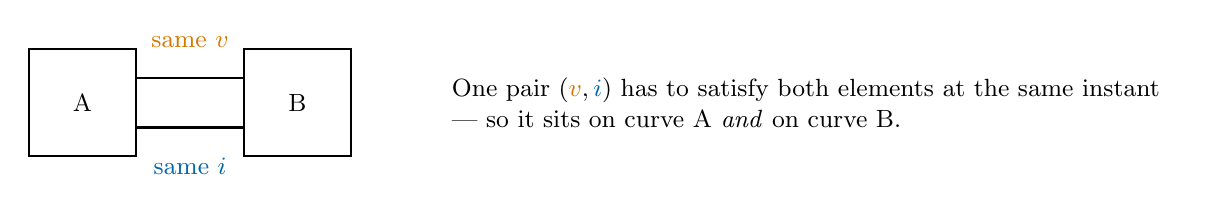
\begin{tikzpicture}[scale=1.05]
  \draw[thick] (0,0) rectangle (1.3,1.3);
  \draw[thick] (2.6,0) rectangle (3.9,1.3);
  \draw[thick] (1.3,0.95) -- (2.6,0.95);
  \draw[thick] (1.3,0.35) -- (2.6,0.35);
  \node[font=\small] at (0.65,0.65) {A};
  \node[font=\small] at (3.25,0.65) {B};
  \node[cvolt, font=\small] at (1.95,1.38) {same $\Vcol{v}$};
  \node[ccur, font=\small] at (1.95,-0.12) {same $\Icol{i}$};
  \node[font=\small, anchor=west, text width=9.4cm] at (5.0,0.65)
    {One pair $(\Vcol{v},\Icol{i})$ has to satisfy both elements at the same instant ---
     so it sits on curve A \emph{and} on curve B.};
\end{tikzpicture}
\end{center}

\begin{examplebox}[Example 3.3 --- a diode driven by a source and a resistor]
A $1.5\V$ source in series with $R$ drives a diode. Walk round the loop with the diode
voltage $\Vcol{v}$ and current $\Icol{i}$:
\[
  \Vcol{v} \;=\; 1.5 - R\,\Icol{i}
  \qquad\Longleftrightarrow\qquad
  \Icol{i} \;=\; \frac{1.5 - \Vcol{v}}{R} .
\]
That is a straight line in the same plane --- the \textbf{load line}. The diode's own
curve is the exponential. The circuit's answer is the single point on both.

\begin{center}
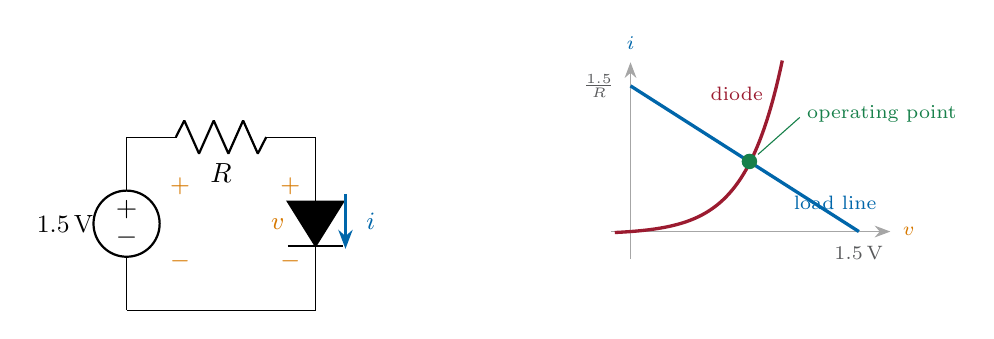
\begin{tikzpicture}[scale=1.0]
\begin{scope}[yshift=0.1cm]
  \draw (0,0) to[american voltage source, invert] (0,2.2);
  \draw (0,2.2) to[R, l_=$R$] (2.4,2.2);
  \draw (2.4,2.2) to[full diode] (2.4,0);
  \draw (2.4,0) -- (0,0);
  \node[pol] at (0.68,1.58) {$+$}; \node[pol] at (0.68,0.62) {$-$};
  \node[font=\small] at (-0.78,1.1) {$1.5\V$};
  \node[pol] at (2.08,1.58) {$+$}; \node[pol] at (2.08,0.62) {$-$};
  \node[pol] at (1.92,1.1) {$v$};
  \draw[iar] (2.78,1.48) -- (2.78,0.78); \node[ccur, font=\small] at (3.1,1.13) {$i$};
\end{scope}
\begin{scope}[xshift=6.4cm, yshift=1.1cm]
  \draw[vax] (-0.25,0) -- (3.3,0) node[right=1pt, font=\scriptsize, text=cvolt] {$v$};
  \draw[vax] (0,-0.35) -- (0,2.15) node[above=1pt, font=\scriptsize, text=ccur] {$i$};
  \draw[crv, domain=-0.2:1.93, samples=170, smooth] plot (\x, {0.035*(exp(2.15*\x)-1)});
  \draw[ccur, very thick] (0,1.85) -- (2.9,0);
  \node[font=\scriptsize, text=ccur] at (2.6,0.36) {load line};
  \node[font=\scriptsize, text=metured] at (1.35,1.75) {diode};
  \fill[cpow] (1.51,0.89) circle (2.8pt);
  \draw[cpow, thin] (1.62,0.98) -- (2.15,1.45);
  \node[font=\scriptsize, text=cpow, right] at (2.12,1.5) {operating point};
  \node[font=\scriptsize, text=metugray, below] at (2.9,-0.06) {$1.5\V$};
  \node[font=\scriptsize, text=metugray, left=1pt] at (-0.04,1.85) {$\frac{1.5}{R}$};
\end{scope}
\end{tikzpicture}
\end{center}
\vspace{-2pt}
Change $R$ and the load line tilts about the point $(1.5\V,\,0)$; change the source and it
slides sideways. The diode's curve never moves. No algebra was needed --- and for a
nonlinear element there often is no algebra to be had.
\end{examplebox}

%==============================================================
\section*{Summary}
\addcontentsline{toc}{section}{Summary}

\begin{itemize}
  \item A two-terminal element is completely described by its \textbf{characteristic}: the
        set of $(\Vcol{v},\Icol{i})$ pairs it permits, drawn as a curve in the
        $v$--$i$ plane.
  \item \textbf{Independent voltage source}: vertical line $\Vcol{v} = v_s(t)$, any
        current. \textbf{Independent current source}: horizontal line $\Icol{i} = i_s(t)$,
        any voltage. Neither one decides the other variable --- the rest of the circuit
        does.
  \item Short circuit $=$ voltage source with $v_s = 0$; open circuit $=$ current source
        with $i_s = 0$.
  \item A \textbf{resistor} is any element whose characteristic is a curve --- an algebraic
        relation, no memory. Diodes and sources are resistors; capacitors and inductors
        are not.
  \item Five questions about the shape of that curve: \textbf{linear} (straight, through
        the origin), \textbf{bilateral} (symmetric about the origin), \textbf{passive}
        (quadrants 1 and 3 only), \textbf{voltage-} or \textbf{current-controlled}
        (single-valued which way round?), \textbf{time-invariant} (does the curve move?).
  \item Where two characteristics cross is where the circuit operates.
\end{itemize}

\subsection*{Next lecture}
Equivalent resistance --- series and parallel combinations and the voltage and current
dividers --- and then the systematic analysis methods.

\subsection*{Reading}
\begin{itemize}
  \item Alexander \& Sadiku, \emph{Fundamentals of Electric Circuits}, Chapter~1--2.
  \item Chua, Desoer \& Kuh, \emph{Linear and Nonlinear Circuits}, Chapter~2 --- the
        closest source to the treatment used here.
  \item Lecture notes and videos of Prof.\ Emre Tuna,
        \href{https://users.metu.edu.tr/etuna/ee201/}{\texttt{users.metu.edu.tr/etuna/ee201}}
        --- Lecture~3 video: voltage source $6{:}50$, current source $16{:}19$,
        activeness $20{:}55$, resistor $22{:}57$, the definitions $33{:}24$--$43{:}10$.
\end{itemize}

\end{document}
